\chapter{Discussion}

\section{Overview}
This section critically examines the key findings, limitations, and challenges encountered throughout the project. The performance of the implemented emotion recognition models is analysed in light of the results obtained, with particular attention given to factors that may have influenced accuracy, generalisability, and reliability. In addition, practical constraints—such as dataset quality, class imbalance, and system implementation limitations—are explored to provide a balanced assessment of the work. Finally, potential improvements and future directions are suggested to address these issues and guide further development.

\section{Face Detection}

The comparative results from the face detection experiments provide valuable insights into the strengths and weaknesses of each model within the context of this project. Notably, the full YOLO model demonstrated superior performance in scenarios involving multiple faces, clearly outperforming its Tiny YOLO counterpart in terms of precision and robustness. However, in simpler cases where only a single face was present, the performance gap between the two models narrowed considerably, with Tiny YOLO showing only a minor drop in average Intersection over Union (IoU) and average precision. This finding supports the hypothesis that Tiny YOLO struggles more with higher-complexity images but remains highly effective for simpler detection tasks.

Given the intended application of this system—namely, a 1-on-1 human-robot interaction scenario—these results suggest that Tiny YOLO offers an efficient and sufficiently accurate solution for real-world deployment. Its lower computational demands make it a practical choice without a significant sacrifice in detection quality for single-face contexts.

In contrast, both the Haar Cascade and HOG+Linear SVM models exhibited a different pattern of strengths. These classical methods outperformed YOLO-based models on the more complex Full Wider Face dataset, particularly in precision. Their high precision but relatively low recall on the full dataset and multiple-face subset indicate a more conservative detection strategy, successfully avoiding false positives but at the cost of missing some true positives. This trade-off highlights their potential utility in applications where false positives must be minimised, although their lower recall limits their suitability for comprehensive face detection tasks.

\section{Facial Emotion Recognition}

A consistent challenge observed across all tested models was the frequent misclassification of sadness as neutral, as highlighted in the confusion matrices. This trend points to a significant limitation in the models' ability to differentiate between these two emotions. Figure \ref{figure:sadneutral} illustrates typical examples of sadness and neutral expressions, emphasizing the subtle visual distinctions between them. This confusion likely stems from the fact that both emotions involve minimal facial muscle movement, lacking the exaggerated features—such as broad smiles or deep frowns—that make other emotions more visually distinct. As a result, even high-performing models struggled to make reliable distinctions in these cases.

\begin{figure}[H]
    \centering{}
    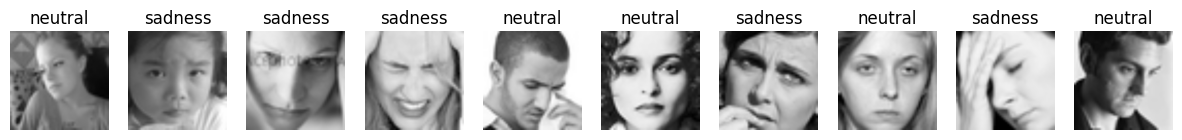
\includegraphics[scale=0.38]{fed_images/sadness+neutral.png}
    \caption{Example images showing the very slight variation between sadness and neutral}
    \label{figure:sadneutral}
\end{figure}

This finding suggests an inherent challenge in relying solely on facial cues for emotion recognition, especially when working with subtle expressions. One potential avenue to mitigate this limitation could involve augmenting training datasets with more diverse and nuanced examples of sadness and neutral expressions, ideally with high-quality labeling to capture fine-grained differences. Alternatively, leveraging the sentiment analysis capabilities of IBM Watson could provide a complementary approach to recognising these specific emotions, particularly in cases where facial cues are ambiguous or difficult to interpret.

A significant limitation encountered during this project relates to the class imbalance present in the facial emotion dataset used for training. The dataset is heavily skewed towards the Happiness (9,355 images) and Neutral (12,905 images) categories, which together account for more than 62\% of the total images. This overrepresentation likely introduced bias into the training process, potentially causing the model to overfit to these dominant classes and reducing its sensitivity to less frequently represented emotions. As noted in previous research \cite{Rangulov2020-pd}, such imbalance can adversely affect the model's generalisability and lead to poor performance when detecting underrepresented emotions.

In contrast, categories such as Contempt (216 images), Disgust (248 images), and Fear (819 images) were severely underrepresented. The limited number of examples in these categories means the model may not have learned the relevant features needed to recognise these emotions reliably. Even emotions like Anger (3,110 images), Sadness (4,370 images), and Surprise (4,462 images), while better represented than the minority classes, still appear in far lower quantities than Happiness and Neutral, which may have resulted in the model's reduced predictive power for these classes

To mitigate this issue in future, several strategies could be employed. One potential solution is the use of data augmentation targeted specifically at the minority classes, rather than on the entire dataset, artificially increasing their representation by generating variations of the existing images through techniques such as rotation, flipping, cropping, or brightness adjustment. Another approach would involve resampling methods—undersampling the overrepresented ones—to achieve a more balanced training set \cite{Mohammed2020-bz}. Alternatively, class weighting \cite{Johnson2019-xc} could have be implemented during training to penalise misclassifications in minority classes more heavily, thereby forcing the model to pay more attention to those examples. In future work, more balanced or curated datasets should be prioritised to help improve overall model performance and robustness across all emotion categories.

\section{Combined Face and Emotion Recognition models}

The results highlight key considerations when selecting face detection and emotion recognition models for real-world robotic systems. Tiny YOLO and full YOLO both provided the highest number of face detections, which directly improved the overall accuracy of emotion recognition when paired with models such as ResNet50. While full YOLO achieved the highest overall accuracy (59.02\%), this came at a significant computational cost, with each face detection taking 0.1610 seconds—over six times slower than Tiny YOLO's 0.0250 seconds. The relatively small gain in accuracy (just 1.66\% higher than Tiny YOLO) raises questions about whether this trade-off is worthwhile in practical applications that require real-time processing.

In terms of emotion recognition, ResNet50 consistently outperformed MobileNetV2 and VGG16 across all face detection methods. However, despite its superior accuracy, ResNet50's high inference time (95.3 milliseconds) and large model size (187MB) introduce challenges, particularly in resource-constrained environments such as mobile robots. By comparison, MobileNetV2 delivered much faster detection times (13.6 milliseconds) and a smaller model size (69.8MB), making it a compelling alternative in situations where speed and memory use are critical concerns. Based on these factors, the combination of Tiny YOLO and MobileNetV2 appeared to offer the best overall balance of accuracy, speed, and memory efficiency, requiring just 92.2MB of memory for both models combined.

A particularly noteworthy finding emerged when these models were deployed on the Turtlebot 4 robot. Here, the performance trends observed during initial tests on the high-powered training PC did not hold: both dlib and Haar Cascade outperformed Tiny YOLO in face detection speed, despite Tiny YOLO being the fastest model during prior evaluations. This shift in performance likely stems from hardware limitations of the Turtlebot 4, which lacks a GPU and has significantly fewer CPU cores than the training machine. These constraints likely prevent Tiny YOLO from leveraging hardware acceleration and parallel processing—key advantages it relies on for fast performance. As a result, its speed advantage diminished in the robot environment.

The emotion recognition models, in contrast, remained consistent across both platforms. MobileNetV2, in particular, maintained its status as the fastest and most efficient option, reinforcing its suitability for deployment in resource-limited robotic systems.

In reflecting on these findings, it is clear that hardware context plays a decisive role in determining which models are optimal. While Tiny YOLO remains the top performer in terms of detection accuracy, its slowed performance on the Turtlebot 4 highlights a key limitation for real-time robotic applications. In scenarios where speed is a higher priority, dlib stands out as the better option despite its lower detection accuracy, while Haar Cascade offers a balanced compromise between speed and performance.

Although the models were ultimately tested in their standard forms, one way to address Tiny YOLO's diminished speed on the robot would have been to explore more hardware-optimised versions of the model, or alternative deployment strategies such as using external compute units, like the Neural Compter Stick 2 or offloading processing to a server. These options could help maintain high accuracy while alleviating on-board resource constraints—an avenue worth considering for future work.

\subsection{Sentiment Discussion}
While the use of a custom, hand-crafted dataset enabled targeted evaluation of IBM Watson's emotion recognition, this method comes with several important limitations. Firstly, the dataset lacks inter-rater reliability; all emotional labels were assigned by a single individual, which introduces subjectivity into the ground truth. In contrast, standardised emotion datasets typically rely on annotations from multiple human raters, reducing personal bias and improving validity.

Secondly, the constructed phrases may overrepresent clear or exaggerated emotional expressions that do not reflect the nuance and ambiguity found in real-world language. As such, the system's strong performance on these examples may not generalise well to less overt emotional content.

Additionally, the small scale of the dataset limits statistical significance and does not support comprehensive evaluation across diverse linguistic contexts. The use of only two examples per emotion class restricts the ability to assess variation within categories or identify borderline or mixed emotional states.

Finally, IBM Watson's emotion analysis API imposes a cap on the number of free requests, meaning large-scale experimentation is not feasible without incurring additional costs. This constraint reinforces the need for a compact, efficient dataset but also limits the scope of evaluation.

The sentiment emotion recognition system has largely met performance expectations, showing robust capabilities in real-time emotion detection. IBM Watson's consistent response times, typically under one second, alongside its reliable accuracy in detecting a range of emotional tones, make it a valuable tool, especially in contexts where facial emotion recognition may not be possible or practical. Its ability to quickly process input and return relevant emotional insights ensures that it can seamlessly complement or even substitute facial emotion recognition when required.

\section{LLM Discussion}

Although the large language model (LLM) component was not responsible for any aspect of emotion recognition, it was tested as part of the system to assess how well it could support natural language interaction. The LLM served as a conversational front-end, providing responses to user inputs that were later analyzed by a separate sentiment analysis tool.

Three models were evaluated for this role — GPT-3.5-turbo, GPT-4o, and GPT-4o-mini — with a focus on response time across a fixed set of phrases. Among the three, GPT-3.5-turbo demonstrated the most consistent and responsive performance, with the lowest average response times and smallest standard deviations across all phrases. This makes it particularly suitable for systems where quick turn-taking is essential. Note, however, that every model exhibited some variability in response times, notably the variation increases as the complexity of the phrases increased. For example, Phrase 1 had an average response time of 0.944 seconds with a standard deviation of 0.067 for GPT-3.5-turbo, while Phrase 9 had an average of 3.166 seconds and a standard deviation of 0.700.

GPT-4o generally offered higher processing times, with occasional latency spikes (e.g., over 5 seconds for Phrase 5), which could interrupt the fluidity of interaction. GPT-4o-mini exhibited similar variability, particularly in later phrases, with average times exceeding six seconds in some cases. This variability may be problematic in real-time applications, particularly on resource-constrained systems.

Given the limited role of the LLM in this architecture — acting purely as a user-facing conversational agent — the results suggest that smaller, faster models like GPT-3.5-turbo are preferable, particularly where consistent, low-latency performance is more important than advanced linguistic ability. These findings help clarify the trade-offs between model complexity and practical responsiveness in a modular system.